%%%%%%%%%%%%%%%%%%%%%%%%%%%%%%%%%%%%%%%%%%%%%%%%%%%%%%%%%%%%%%%%%%%%%%
% How to use writeLaTeX: 
%
% You edit the source code here on the left, and the preview on the
% right shows you the result within a few seconds.
%
% Bookmark this page and share the URL with your co-authors. They can
% edit at the same time!
%
% You can upload figures, bibliographies, custom classes and
% styles using the files menu.
%
%%%%%%%%%%%%%%%%%%%%%%%%%%%%%%%%%%%%%%%%%%%%%%%%%%%%%%%%%%%%%%%%%%%%%%

\documentclass[12pt]{article}

\usepackage{sbc-template}

\usepackage{graphicx,url}

%\usepackage[brazil]{babel}   
\usepackage[utf8]{inputenc}  
\usepackage{subfig}
    
\sloppy

\title{Minimização de Automatos Finitos\\ Deterministicos}

\author{July F. M. Werneckl\inst{1}, Thiago Amado Costa\inst{2} }


\address{Instituto de Ciências Exatas e 
Informática -- Pontifícia Universidade Católica \\de 
Minas Gerais\\
  Belo Horizonte, Minas Gerais
\nextinstitute
  Instituto de Ciências Exatas e 
Informática -- Pontifícia Universidade Católica \\de 
Minas Gerais\\
  Belo Horizonte, Minas Gerais
% \nextinstitute
%   Departamento de Sistemas e Computação\\
%   Universidade Regional de Blumenal (FURB) -- Blumenau, SC -- Brazil
  \email{\{jfmwerneck@sga.pucminas.br, thiago.amado@sga.pucminas.br}
}

\begin{document} 

\maketitle

% \begin{abstract}
%   This meta-paper describes the style to be used in articles and short papers
%   for SBC conferences. For papers in English, you should add just an abstract
%   while for the papers in Portuguese, we also ask for an abstract in
%   Portuguese (``resumo''). In both cases, abstracts should not have more than
%   10 lines and must be in the first page of the paper.
% \end{abstract}
     
\begin{resumo} 
Este artigo descreve a implementação de dois métodos de minimização de Automatos Finitos Determinísticos, o método $O(n^2)$, encontrado em livros didáticos, e o método $O(n \log{}n)$, inicialmente proposto por \cite{hopcroft1971n}. \\Ambos métodos foram implementados seguindo a apresentação de \cite{blum1996n}.
\end{resumo}


\section{Introdução}

De acordo com a definição dada por \cite{vieira2006introduccao}, um $AFD M$ é mínimo para a linguagem $L(m)$ se nenhum $AFD$ para $L(m)$ contém menor número de estados que $M$. Dessa forma, para construir um $AFD$ minimo, o primeiro passo é remover os estados inalcançáveis a partir do inicial, e em seguida, determinar quais estados são equivalentes, para então reconstruir a função de transição. Os algoritmos em análise se diferem principalmente etapa de verificação de estados equivalentes. 

\section{Implementação}

Os algoritmos propostos foram reescritos na linguagem Python. Os arquivos de entrada e saída seguem o formato adotado pelo simulador JFLAP versão 7.0 para a descrição do Autômato. Todos os testes e autômatos de entrada estão na pasta ./tests/, e resultados na pasta ./results/.
\\
Para a leitura do arquivo de entrada, foi implementada uma função que obtém da entrada o conjunto de estados ($E$), transições ($\delta$) e alfabeto ($\sum$) , além do estado inicial($i$) e conjunto de estados finais ($F$), resultando em um automato finito $P = (E, \sum, \delta, i ,F )$.
\\
Após a obtenção do autômato, são retirados do mesmo os estados inalcançáveis a partir do inicial, para então ser minimizado.
\\
A seguir, a descrição dos métodos implementados:

\subsection{Método $O(n^2)$}
O algoritmo para minimização do autômato está contido em uma função denominada $min\textunderscore nn$ no 
arquivo $Minimize.py$ A função recebe como parâmetro um autômato $P$ do tipo AFD, classe 
auxiliar para a implementação de todo o código. 

Dentro de $min\textunderscore nn$, temos uma função encapsulada $\textunderscore get\textunderscore set\textunderscore c\textunderscore transition$ que recebe como 
parâmetro um $_S$, variável que armazena as partições, e também um estado $\textunderscore e$. A função tem 
como objetivo auxiliar na determinação de qual partição um estado está contido, e por 
isso retorna $i$, que contém essa informação. 

As duas primeiras verificações do processo de minimização são para definir se o autômato 
$P$ recebido como parâmetro possui algum estado final, e também, se todos os estados são 
finais, já que em ambos os casos, por definição, o autômato minimizado seria um único 
estado com todas as transições do alfabeto para ele mesmo. 

Caso nenhuma condicional seja satisfeita, criamos duas variáveis, sendo $S$ o vetor que 
armazena as diferentes partições, e $n$ uma variável inteira que vai acessar os índices de 
$S$, inicializada com 0. Além disso, inicializamos $S$ dividindo os estados de $P$ em finais e 
não finais, desta forma $S[0]$ possui uma partição contendo todos os estados não finais e 
outra partição com todos os finais. 

No próximo passo, temos um while que executa enquanto o tamanho de $S$ for igual a um ou 
enquanto o $S$ atual for diferente do $S$ anterior. Uma vez dentro do loop incrementamos a 
variável $n$ em uma unidade e chegamos em um loop for que itera sobre as partições $X$ de $S$, 
enquanto existirem partições não vazias, faz-se: 
\begin{enumerate}
    \item Pegamos o estado $e$ presente na primeira posição da partição X, e para cada símbolo do alfabeto verificamos qual estado é alcançado por $e$ com o símbolo $a$, com auxílio do método contido na classe P $get\textunderscore reachable\textunderscore state\textunderscore by\textunderscore symbol$ que pode ser expressado por $\delta$(e, a) = $reachable\textunderscore state$. Em seguida, utilizamos a função encapsulada descrita anteriormente para acessar em qual das partições de $S$ o resultado da transição está contido, armazenando-o em uma variável denominada $transitions\textunderscore set$[a]. 
    \item Uma vez terminado os símbolos do alfabeto, criamos uma variável Y e a inicializamos com o estado $e$, entramos em um for que vai verificar se os estados $\textunderscore e$ que fazem parte da mesma partição $X$ de $e$, possuem transição para mesma partição armazenada em $transitions\textunderscore set$, com todos os símbolos do alfabeto. Para determinar se $\textunderscore e$ deve continuar na mesma partição de $e$, utilizamos um contador $count$ que é incrementado em um cada vez que a expressão é satisfeita $\delta$(\textunderscore $e, b)$ $\in$ $transitions\textunderscore set[b]$, caso count seja igual ao total de símbolos no alfabeto então adicionamos \textunderscore $e$ em $Y$.
    \item Em seguida, atualizamos $X$ para $X$ - $Y$ e adicionamos $Y$ em $S[n]$.
\end{enumerate}

Ao sairmos do while mais exterior, temos a certeza que foi definido quais os estados 
são correspondentes e consequentemente temos o autômato minimizado. 

Os passos seguintes são responsáveis por reconstruir o autômato, definindo que, caso uma partição contenha um símbolo inicial, portanto esta é inicial, seguimos a mesma lógica para definição de quais os novos estados de aceite. Já para transições, utilizamos a combinação da função 
$get\textunderscore reachable\textunderscore state\textunderscore by\textunderscore symbol$ e a $\textunderscore get\textunderscore set\textunderscore c\textunderscore transition$ para definir em qual partição 
está o resultado de uma transição antiga. Finalmente, temos o autômato devidamente 
minimizado e equivalente a $P$. 

\subsection{Método $O(n \log{} n)$}
O algoritmo para minimização do autômato está contido em uma função denominada $min\textunderscore nlogn$ no arquivo $Minimize.py$. Para implementação do mesmo, como citado anteriormente, utilizamos alguma estruturas complementares que garantem o ganho de tempo computacional, sendo elas: 

$L[i, a, j]$: estrutura que armazena quais estados da partição $i$ alcançam a partição $j$ com o símbolo $a$;

$triangle(q, a)$: armazena o identificador da lista que contém o resultado da transição $\delta$(q, a), em que $q$ é um estado e $a$ um símbolo;

$inverted\textunderscore triangle(b, q)$: lista de estados que alcançam o estado $q$ com símbolo $b$;

$\textunderscore triangle(i, a)$: armazena o identificador da lista que contém as relações da partição $i$ com o símbolo $a$;

$K$: dicionário que contem a relação entre a chave de \textunderscore $triangle$ que armazena mais que um identificador de lista.

Os primeiros passos da implementação são dedicados à construção das estruturas auxiliares citadas acima, a execução do algoritmo ocorre majoritariamente em função do $K$ já que este contém as partições que com um mesmo símbolo vão para partições diferentes. E por isso, enquanto K não estiver vazio, executamos os passos: 
\begin{enumerate}
    \item Para cada relação $\textunderscore triangle$ contida em $K$, pegamos duas triplas $L(i, a, j_1)$ e $L(i, a, j_2)$, escolhemos a menor lista e a transformamos em uma nova lista $L(t, a, j_{min})$. Note que neste ponto, não utilizamos $t+1$ pois nosso $t$ já é inicializado com dois. Então, atualizamos as estruturas adjacentes para a nova partição criada, deletando a ocorrência da lista $L(i, a, j_{min})$ de $\textunderscore triangle$ e adicionando a nova lista, e ainda, caso a lista remanescente de $\textunderscore triangle(i, a)$ for menor que dois, deletamos sua ocorrência de $K$. 
    \item Para cada estado $q$ contido na nova lista $L(t, a, j_{min})$ vamos atualizar as demais estruturas para nova partição que fazem parte:
    \begin{enumerate}
        \item Para cada símbolo $b$ do alfabeto, sendo $b$ != $a$, utilizamos $triangle(q, b)$ para encontrar a lista $L(i, b, k)$ que armazena o resultado da transição, que pode ser expressada por $\delta$(q, b) = result. Removemos result da lista anterior e adicionamos a nova lista, $L(new\textunderscore ibk)$, adicionalmente, atualizamos também a estrutura $triangle$. Caso a lista antiga fique vazia, removemos sua ocorrência nas demais estruturas, conforme necessário. Ainda, adicionamos $L(new\textunderscore ibk)$ em $\textunderscore triangle(t, b)$ e eventualmente, em $K$, caso a lista torne-se maior que um. 
        \item Para todos os símbolos do alfabeto, utilizamos a estrutura do $inverted\textunderscore triangle$ para obter quais estados, $p$, alcançavam a antiga partição, e a partir de $triangle$ obtemos o identificador da lista $L(k, b, i)$ que deve ser modificado para nova partição criada. Dessa forma, removemos $p$ da antiga lista e inserimos em $L(new\textunderscore kbt)$. Atualizamos as estruturas adjacentes seguindo a mesma lógica do passo anterior.
        \item Ao final, sempre incrementamos a variável $t$ em uma unidade.
    \end{enumerate}
\end{enumerate}  

Para definição dos estados iniciais e finais do $AFD-M$ utilizamos a mesma lógica do método $n^2$, já para definição das transições iteramos sobre as chaves de $L$ e obtemos a relação de cada partição com os símbolos do alfabeto. 

Ao final do algoritmo, obtemos as partições separando corretamente os estados e os relacionando de acordo com as transições iniciais, por isso, obtemos um AFD equivalente e mínimo ao P de origem. 

\section{Experimentos e Resultados}\label{sec:figs}

Inicialmente, foi testado o funcionamento dos algoritmos com o autômato que identifica binários módulo 6 (Figura 1a), proposto em \cite{vieira2006introduccao}, e um autômato que pode ser definido pela seguinte expressão regular $ER = (1 \cup 01^*01^*01^*01^*01^*01^*01^*01^*01^*0)^*$ (Figura 1b)


% \begin{figure}[ht]
% \centering
% 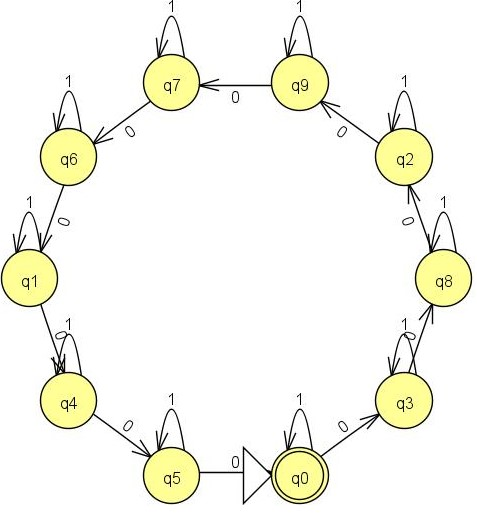
\includegraphics[width=.5\textwidth]{images/automato2.jpg}
% \caption{Fecho de 0 e 1}
% \label{fig:automato2}
% \end{figure}

\begin{figure}[ht]
  \centering
  \subfloat[Figura 1: Binário mod 6]{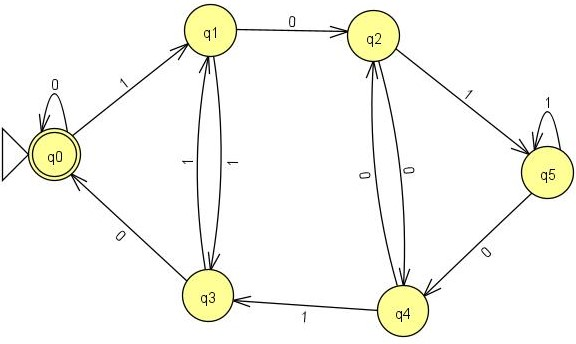
\includegraphics[width=0.6\textwidth]{images/automato1.jpg} \label{fig:automato1}} 
  \\
  \subfloat[Figura 1: $(1 \cup (01^*)^9)^*$]{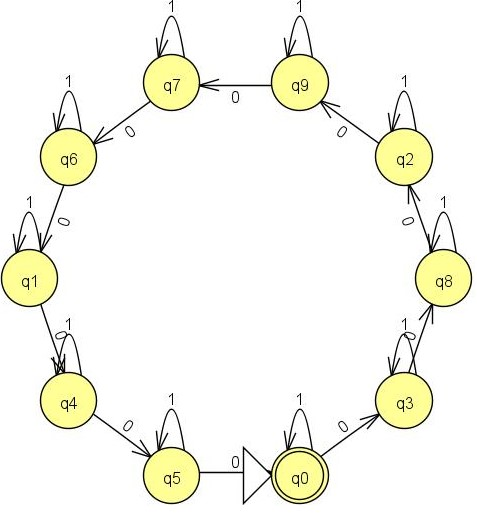
\includegraphics[width=0.5\textwidth]{images/automato2.jpg} \label{fig:automato2}}
\end{figure}

\subsection{Teste 1}

Utilizando o autômato da Figura 1a, ambos algoritmos obtiveram AFDs mínimos equivalentes. O método $O(n^2)$ resultou no AFD representado na Figura 2a, e o método $O(n \log{} n)$ resultou no AFD representado na Figura 2b.
O autômato em questão representa um caso médio, portanto, ambos algoritmos obtiveram resultados semelhantes em tempo de execução.

\begin{figure}[ht]
  \centering
  \subfloat[Figura 2: Resultado do algoritmo ($O(n^2)$)]{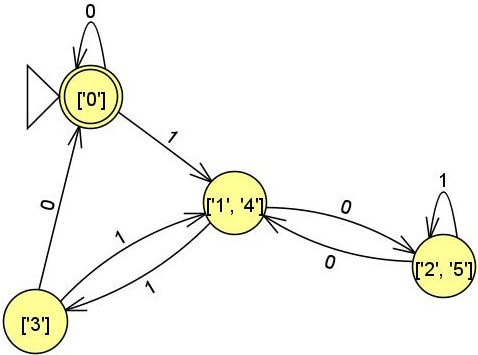
\includegraphics[width=0.6\textwidth]{images/min_automato1_n2.jpg} \label{fig:automato1_n2}} 
  \\
  \subfloat[Figura 2: Resultado do algoritmo ($O(n \log{} n)$)]{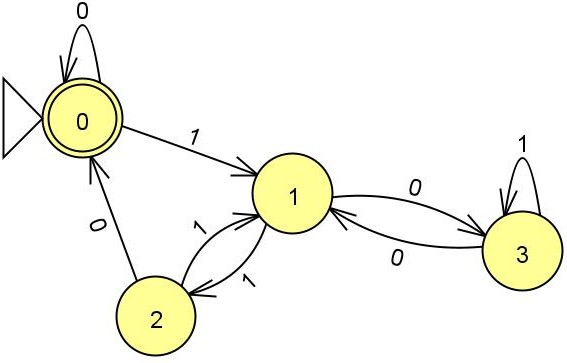
\includegraphics[width=0.5\textwidth]{images/min_automato1_nlogn.jpg} \label{fig:automato1_nlogn}}
\end{figure}

\subsection{Teste 2}
Utilizando o autômato da Figura 1b, ambos algoritmos obtiveram AFDs mínimos equivalentes. O método $O(n^2)$ resultou no AFD da Figura 3a, e o método $O(n\log{}n)$ resultou no AFD da Figura 3b.
\\
No autômato em questão nenhum estado é equivalente a outro, fazendo-se necessário que o algoritmo gere K partições, em que K = numero de estados. Assim, era esperado que os algoritmos tivessem tempos de execução diferentes, porém, ambos algoritmos obtiveram tempos semelhantes de execução, fazendo-se necessário testes com mais estados para observar maiores diferenças.
% forçar imagem na section certa
\\ 
\\ 
\\ 
\\
\\
\\
\\
\\

\begin{figure}[ht!]
  \centering
  \subfloat[Figura 3: AFD mínimo ($O(n^2)$)]{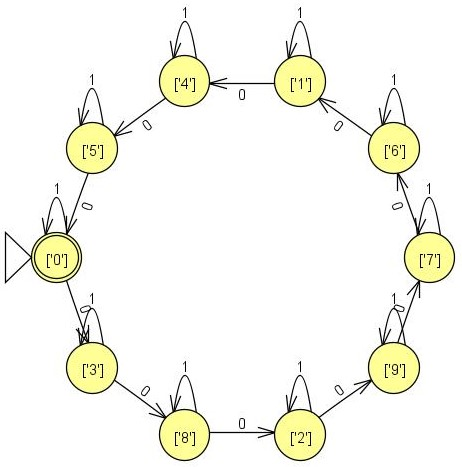
\includegraphics[width=0.5\textwidth]{images/min_automato2_nn.jpg} \label{fig:automato2_n2}} 
  \\
  \subfloat[Figura 3: AFD mínimo ($O(n \log{} n)$)]{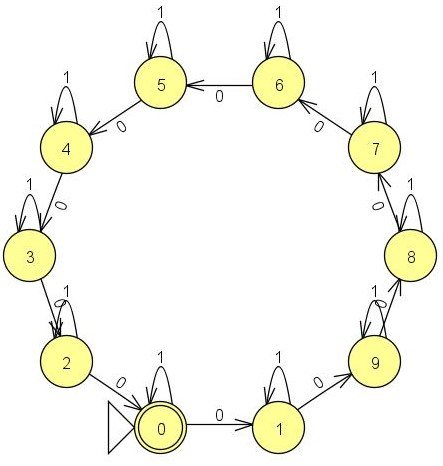
\includegraphics[width=0.5\textwidth]{images/min_automato2_nlogn.jpg} \label{fig:automato2_nlogn}}
\end{figure}


\subsection{Testes Finais}
Seguindo o padrão do autômato representado na Figura 1b,em que cada estado possui uma transição para si mesmo com 1 e uma transição para o próximo com 0, foram criados 4 autômatos, com o numero de estados em 100, 500, 1000 e 2000 estados.
A seguir, segue uma tabela contendo uma média dos tempos de execução, em segundos, de cada algoritmo, para cada um dos 4 autômatos. 
% forçar table na section certa
\\  
\\
\\

\begin{table}[ht!]
\begin{center}   
\begin{tabular}{|l|l|l|}
\hline
\textbf{n} & \textbf{$0(n^2)$} & \textit{\textbf{$O(n log{}n)$}} \\ \hline
100        & 0.028             & 0.002                           \\ \hline
500        & 2.56              & 0.033                           \\ \hline
1000       & 17.70             & 0.12                            \\ \hline
2000       & 135.20            & 0.48                            \\ \hline
\end{tabular}
\end{center}
\end{table}


\section{Conclusão}

Observando a tabela com as médias de tempo de execução para cada algoritmo, fica claro que o Teorema 1 proposto por \cite{blum1996n} vale. É possível observar a partir dos testes finais que a diferença entre o tempo de execução das duas implementações cresce a medida que o número de estados aumenta. Para estados menores ou iguais a 100 a diferença é relativamente similar, considerando a perspectiva humana, e por isso, para estes casos o implementação $n^2$ deve ser suficientemente boa. Já a implementação nlogn ganha destaque para autômatos grandes e cenários em que milésimos fazem diferença. 
A implementação cuja complexidade é nlogn constrói sua vantagem na criação de estruturas auxiliares para determinação de diferentes partições, sendo assim uma solução de compromisso entre a memória utilizada e o tempo de execução para determinar um autômato minimizado. 

\bibliographystyle{sbc}
\bibliography{sbc-template}

\end{document}
